% $Header: /home/vedranm/bitbucket/beamer/solutions/conference-talks/conference-ornate-20min.en.tex,v 90e850259b8b 2007/01/28 20:48:30 tantau $

\documentclass[xcolor=dvipsnames]{beamer} 

\usepackage{ulem}


% This file is a solution template for:

% - Talk at a conference/colloquium.
% - Talk length is about 20min.
% - Style is ornate.



% Copyright 2004 by Till Tantau <tantau@users.sourceforge.net>.
%
% In principle, this file can be redistributed and/or modified under
% the terms of the GNU Public License, version 2.
%
% However, this file is supposed to be a template to be modified
% for your own needs. For this reason, if you use this file as a
% template and not specifically distribute it as part of a another
% package/program, I grant the extra permission to freely copy and
% modify this file as you see fit and even to delete this copyright
% notice. 


\mode<presentation>
{
  %\usetheme{boxes}
  %\usecolortheme{seagull}
  % or ...

  \setbeamercovered{transparent}
  % or whatever (possibly just delete it)

    \usecolortheme[named=OliveGreen]{structure} 
    \usetheme[height=7mm]{Rochester} 
    \setbeamertemplate{items}[ball] 
    \setbeamertemplate{blocks}[rounded][shadow=true]
}


\usepackage[czech]{babel}
% or whatever

\usepackage[utf8]{inputenc}
% or whatever

\usepackage{hyperref}
%\definecolor{links}{HTML}{2A1B81}
\hypersetup{colorlinks,linkcolor=OliveGreen,urlcolor=OliveGreen}

\usepackage{times}
% \usepackage[T1]{fontenc}
% Or whatever. Note that the encoding and the font should match. If T1
% does not look nice, try deleting the line with the fontenc.


\title[OpenStreetMap] % (optional, use only with long paper titles)
{OpenStreetMap}

\subtitle {Wiki-pohled na Geodata}

\author[J. Čepický] % (optional, use only with lots of authors)
{Jáchym~Čepický\inst{1}\inst{2}}
% - Give the names in the same order as the appear in the paper.
% - Use the \inst{?} command only if the authors have different
%   affiliation.

\institute % (optional, but mostly needed)
{
  \inst{1}%
  Open Source Geospatial Foundation
  \url{http://osgeo.org}\\

  \inst{2}%
  Geosense s.r.o.
  \url{http://geosense.cz}\\
}
  
% - Use the \inst command only if there are several affiliations.
% - Keep it simple, no one is interested in your street address.

\date[] % (optional, should be abbreviation of conference name)
{Wikikonference 2013, Praha}
% - Either use conference name or its abbreviation.
% - Not really informative to the audience, more for people (including
%   yourself) who are reading the slides online

% If you have a file called "university-logo-filename.xxx", where xxx
% is a graphic format that can be processed by latex or pdflatex,
% resp., then you can add a logo as follows:

\pgfdeclareimage[height=1.cm]{conference-logo}{images/220px-Wikimedia_Czech_Republic-logo.svg.png}
\pgfdeclareimage[height=1.cm]{osm-logo}{images/osm_logo-79d71f6a51b0e6a724a570834c07d828.png}
\logo{\pgfuseimage{conference-logo}}



% Delete this, if you do not want the table of contents to pop up at
% the beginning of each subsection:
\AtBeginSection[]
{
\logo{\pgfuseimage{conference-logo}}
  \begin{frame}<beamer>{TOC}
    \tableofcontents[currentsection,currentsubsection]
  \end{frame}
}


% If you wish to uncover everything in a step-wise fashion, uncomment
% the following command: 

%\beamerdefaultoverlayspecification{<+->}


\begin{document}

\begin{frame}
  \titlepage
\end{frame}


% Structuring a talk is a difficult task and the following structure
% may not be suitable. Here are some rules that apply for this
% solution: 

% - Exactly two or three sections (other than the summary).
% - At *most* three subsections per section.
% - Talk about 30s to 2min per frame. So there should be between about
%   15 and 30 frames, all told.

% - A conference audience is likely to know very little of what you
%   are going to talk about. So *simplify*!
% - In a 20min talk, getting the main ideas across is hard
%   enough. Leave out details, even if it means being less precise than
%   you think necessary.
% - If you omit details that are vital to the proof/implementation,
%   just say so once. Everybody will be happy with that.


\begin{frame}{Jak začít s editací}
\begin{itemize}
    \item Přihlásit se do OSM
    \item Přihlásit se do talk-cz
    \item Stáhnout editor
    \item Podívejte se na features \href{http://wiki.openstreetmap.org/wiki/Map\_Features}{http://wiki.openstreetmap.org/wiki/Map\_Features}
    \item OpenStreetBugs (nyní na hlavní stránce)
\end{itemize}
\end{frame}

\begin{frame}{Editory}
    \begin{center}
    \only<1>{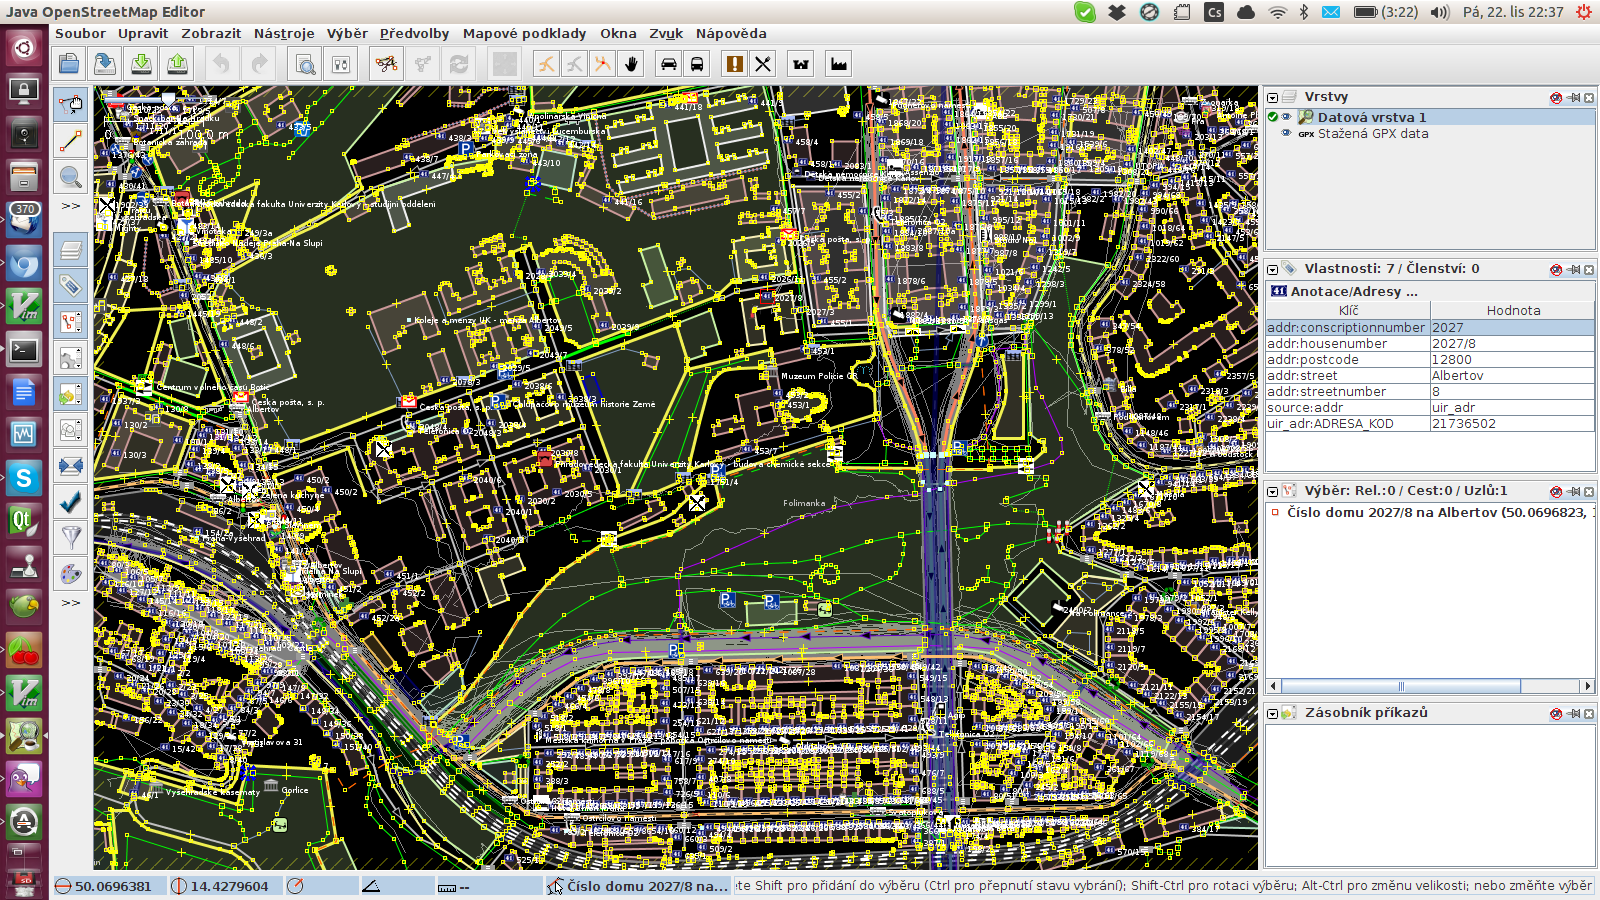
\includegraphics[width=\textwidth]{images/josm-edit.png}}
    \only<2>{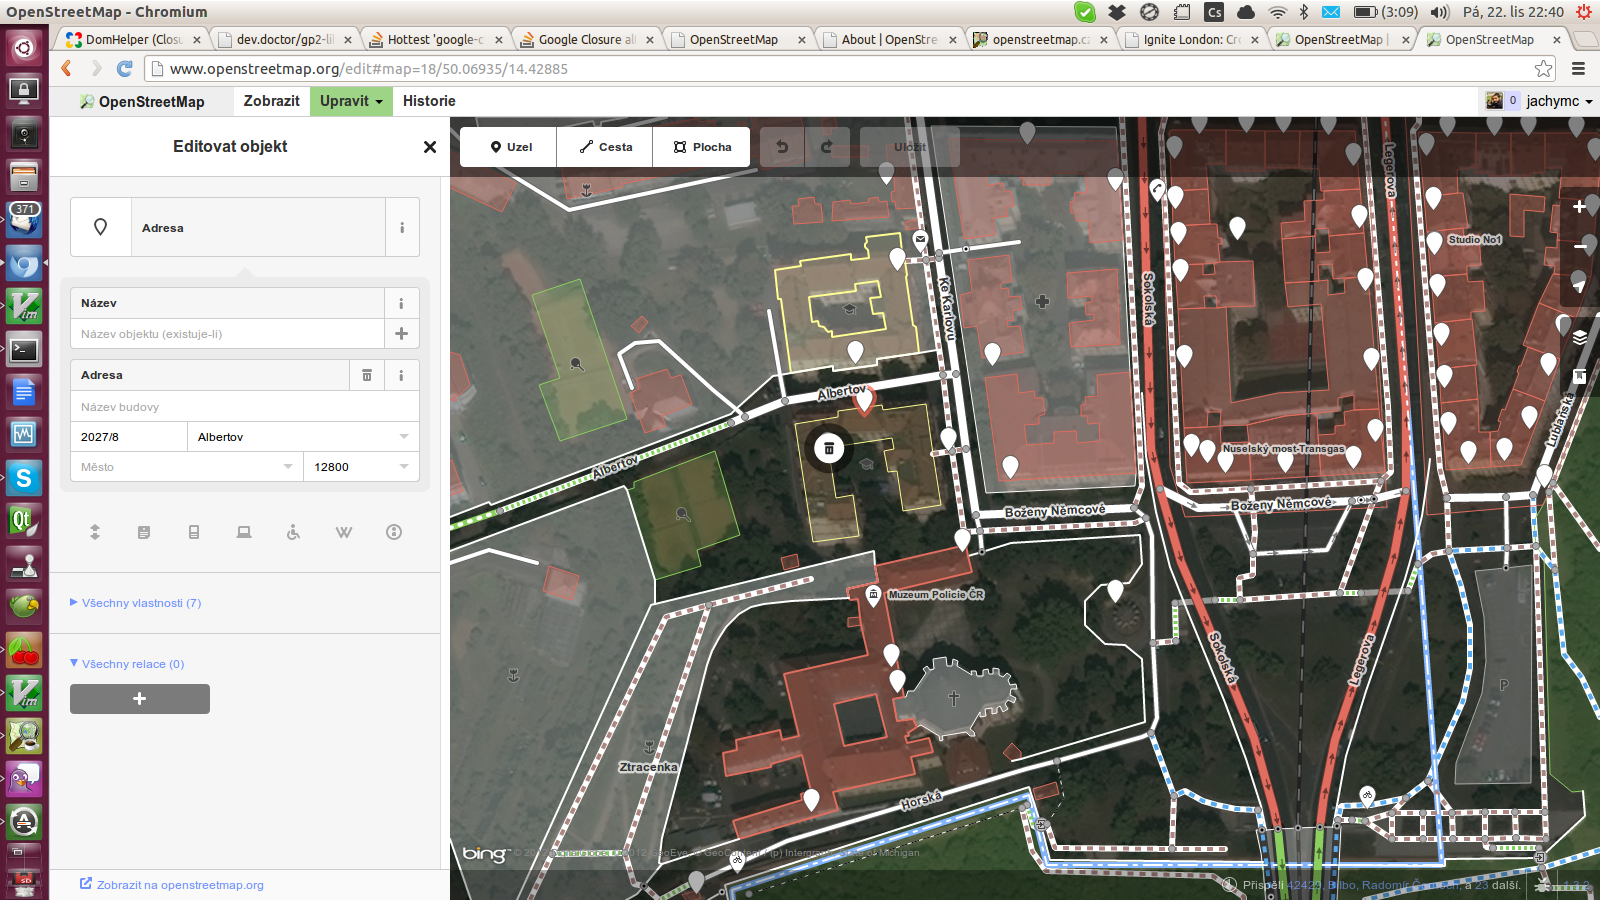
\includegraphics[width=\textwidth]{images/id-edit.png}}
    \end{center}
\end{frame}

\begin{frame}{Používání dat}
\begin{itemize}
    \item OSM API
    \item download.geofabrik.de
\end{itemize}
\end{frame}

\begin{frame}{Související}
\begin{itemize}
    \item Prahou na kole
    \item OpenAerialMap
    \item GrassRootsMapping
    \item Mapbox
    \item \href{http://osmbuildings.org}{http://osmbuildings.org}  a další
\end{itemize}
\end{frame}


\begin{frame}{Další}
\begin{itemize}
    \item
    \href{http://wiki.openstreetmap.org/wiki/Quality\_assurance}{http://wiki.openstreetmap.org/wiki/Quality\_assurance}
    \item Datareport 2013 \href{https://www.mapbox.com/osm-data-report/}{https://www.mapbox.com/osm-data-report/}
        \begin{itemize}
            \item Přes 1~000~000 přispěvatelů
            \item 78~000~000 budov, 33~000~00 km cest
            \item Update každou 1s \href{https://www.mapbox.com/openstreetmap/}{https://www.mapbox.com/openstreetmap/}
        \end{itemize}
\end{itemize}
\end{frame}


\end{document}


